% =====================================================================
\chapter{Implementation}
\label{ch:impl}
% =====================================================================

This chapter describes how \veriscript{} was implemented and how the
experiments were set up: the algorithms and techniques used in each module,
the software tools and hardware, the hyperparameters that were searched and
selected, the latency measurement protocol, and the corpus that was built from
public benchmarks. It then presents the code organisation, key implementation
excerpts, the training runs, the user interfaces and the testing strategy, and
closes with the completed work plan and a list of the points on which the
implementation differs from the plan of Chapters~3--5. All numbers in this
chapter come from the actual runs; the results of the evaluation are analysed
in Chapter~\ref{ch:results}.

% ---------------------------------------------------------------------
\section{Experimental Setup}
% ---------------------------------------------------------------------

\subsection{Algorithms and Techniques Used}

\subsubsection{Reference Language Model Scoring}

The perplexity, rank and entropy features of the heuristic stage are
computed with GPT-2 small~\cite{radford2019language} (124.4 million
parameters), loaded through the Hugging Face Transformers
library~\cite{wolf2020transformers}. A document is tokenised with the GPT-2
byte-pair-encoding tokeniser and scored in chunks of at most 1023 tokens, each
prefixed with the beginning-of-text token so that the first word of every
chunk is also predicted; at most 2048 tokens of a document are scored. For
each position $i$, the log-softmax of the output logits gives
$\log P(x_i \mid x_{<i})$ for the observed token, its rank among all 50,257
vocabulary entries, and the entropy $H_i$ of Eq.~\eqref{eq:entropy}. The
character offsets returned by the tokeniser are mapped onto the sentence spans
produced by the pre-processor, so that per-sentence perplexities can be
aggregated over sentences of at least five tokens. Perplexities are clipped at
$10^4$ so that a single garbled sentence cannot dominate the feature. GPT-2
small is used because it is openly licensed, is the reference model of
GLTR~\cite{gehrmann2019gltr}, and is different from the generators being
detected: the heuristic stage must not depend on access to the generator. On
the GPU the model runs in half precision.

\subsubsection{Sentence Segmentation and Part-of-Speech Tagging}

spaCy's small English pipeline (\texttt{en\_core\_web\_sm}~3.8) provides
sentence boundaries (statistical sentence recogniser) and universal
part-of-speech tags. The parser, lemmatiser and named-entity recogniser are
disabled because they are not needed. The POS-bigram profile counts every
bigram of universal tags inside a sentence and normalises by the total count;
the 20 bigrams retained as features are those with the highest mutual
information with the label on the training split. A regular-expression
sentence splitter is used as a fall-back when spaCy is unavailable.

\subsubsection{Logistic Regression}

Logistic regression models the log-odds of the AI class as a linear function
of the standardised features (Eq.~\eqref{eq:lr}). It is trained with the
L-BFGS solver in scikit-learn~\cite{pedregosa2011sklearn}, with the inverse
regularisation strength $C$ chosen by five-fold stratified cross-validation
(scoring AUROC) from $\{0.01, 0.1, 1, 10\}$. Its advantages are speed,
stability on small feature sets and the exact additive explanation described
in Chapter~\ref{ch:proposed}.

\subsubsection{Gradient-Boosted Decision Trees}

Gradient boosting builds an additive ensemble of shallow regression trees,
each fitted to the negative gradient of the loss of the current ensemble
(Eq.~\eqref{eq:gbdt}). The XGBoost implementation~\cite{chen2016xgboost} is
used with histogram-based tree construction. Twelve configurations are drawn
at random from a grid over maximum depth $\{3,\dots,6\}$, learning rate
$\{0.03, 0.05, 0.1\}$, minimum child weight $\{1,3,5\}$ and $\ell_2$ penalty
$\{1,3,10\}$; each is trained with up to 800 trees and early stopping after 50
rounds without improvement of the validation log-loss, and the configuration
with the highest validation AUROC is kept. Per-feature contributions for
explanations are obtained with XGBoost's path-based attribution
(\texttt{pred\_contribs}).

\subsubsection{Probability Calibration}

Two calibrators are fitted on the calibration split to the raw log-odds score
of the selected head: Platt scaling~\cite{platt1999probabilistic}, a
one-dimensional logistic regression (Eq.~\eqref{eq:platt}), and isotonic
regression, a non-decreasing step function fitted by the
pool-adjacent-violators algorithm. The calibrator with the lower expected
calibration error (Eq.~\eqref{eq:ece}, ten equal-width bins) on the validation
split is retained. The uncalibrated sigmoid of the raw score is also stored for
every document so that the effect of calibration (RQ2) can be measured.

\subsubsection{Transformer Fine-Tuning}

RoBERTa-base~\cite{liu2019roberta} (124.6 million parameters including the
classification head) is fine-tuned with a two-class sequence-classification
head using PyTorch~\cite{paszke2019pytorch} and the Transformers
\texttt{Trainer} API. Optimisation uses AdamW~\cite{loshchilov2019adamw} with a
linear warm-up over the first 6\% of steps followed by linear decay, mixed
precision (FP16), evaluation after every epoch and early stopping on
validation F1 with a patience of one epoch; the best checkpoint is restored at
the end. Training documents are truncated to their first 512 tokens. At
inference, documents longer than 512 tokens are processed in windows of 510
content tokens whose start positions are 384 tokens apart, the windows are
sorted by length and scored in mini-batches, and the window probabilities are
averaged (Eq.~\eqref{eq:windows}). DeBERTa-v3-base~\cite{he2023debertav3} is
supported by the same script (\texttt{--model microsoft/deberta-v3-base},
trained in full precision because DeBERTa-v3 is unstable in FP16).

\subsubsection{Threshold Search}

The ambiguity band is selected by the exhaustive grid search of
Algorithm~\ref{alg:tune} with a step of 0.01, giving $51 \times 51 = 2601$
candidate bands. Because the predictions of both stages on the validation set
and on the fairness validation set are computed once and cached, the search
evaluates all candidates at once with vectorised NumPy operations in under a
second. Three operating points are produced from the same search with
different accuracy tolerances: \emph{thorough} ($\varepsilon=0.005$),
\emph{balanced} ($\varepsilon=0.02$, the value fixed in Table~\ref{tab:gap-obj})
and \emph{fast} ($\varepsilon=0.05$).

\subsubsection{Evaluation Techniques}

Accuracy is measured with Accuracy, Precision, Recall, F1, AUROC, the false
positive rate and the expected calibration error. 95\% confidence intervals for
F1 and AUROC are estimated by percentile bootstrap resampling of the test set
(1000 resamples). The difference between the cascade and each baseline is
tested with a paired bootstrap on identical resamples. For cross-generator
generalisation, one family (Mistral) is excluded from the whole pipeline and
forms its own test set; in addition, the heuristic stage is retrained seven
more times, each time without one of the remaining families, and a second
RoBERTa model is fine-tuned without the Llama family so that the full cascade
can also be evaluated under the leave-one-generator-out protocol. For
fairness, the false positive rate is computed separately on native and
non-native human-written essays. Chapter~\ref{ch:results} defines all
measures formally.

\subsection{Software Tools Used}

Table~\ref{tab:software} lists the software used, with the exact versions of
the environment in which all reported results were produced. All tools are
open source.

\begin{table}[H]
\caption{Software tools and libraries}
\label{tab:software}
\centering
\small
\begin{tabularx}{\textwidth}{|p{3.9cm}|p{1.9cm}|L|}
\hline
\textbf{Tool / library} & \textbf{Version} & \textbf{Purpose} \\ \hline
Python & 3.11.7 & Implementation language \\ \hline
PyTorch~\cite{paszke2019pytorch} & 2.5.1 (CUDA 12.4) & Tensor computation, GPU training and inference \\ \hline
Hugging Face Transformers~\cite{wolf2020transformers} & 4.46.3 & GPT-2 and RoBERTa models, tokenisers, \texttt{Trainer} \\ \hline
Hugging Face Datasets / Hub & 3.1.0 & Tokenised training sets; downloading benchmark files \\ \hline
scikit-learn~\cite{pedregosa2011sklearn} & 1.5.2 & Logistic regression, isotonic regression, mutual information, metrics \\ \hline
XGBoost~\cite{chen2016xgboost} & 2.1.3 & Gradient-boosted trees, path-based attributions \\ \hline
spaCy (\texttt{en\_core\_web\_sm}) & 3.8.2 (3.8.0) & Sentence segmentation and part-of-speech tagging \\ \hline
NumPy, pandas, PyArrow & 1.26, 2.2, 17.0 & Feature matrices, Parquet storage, vectorised threshold search \\ \hline
SciPy & 1.17 & Rank statistics for bootstrap AUROC \\ \hline
Matplotlib & 3.11 & ROC, calibration, trade-off and result plots \\ \hline
pdfplumber, python-docx & 0.11, 1.2 & Text extraction from PDF and Word files \\ \hline
FastAPI, Uvicorn & 0.115, 0.32 & REST service \\ \hline
Streamlit & 1.40.2 & Web interface \\ \hline
Typer & 0.13.1 & \texttt{veriscript} command line tool \\ \hline
pytest & 9.2 & Unit, integration and API tests \\ \hline
Docker & 28.3 & Container image for deployment \\ \hline
Git & -- & Version control \\ \hline
\end{tabularx}
\end{table}

\textbf{PyTorch and Transformers} provide the neural models and give a
uniform interface to GPT-2 (for the reference statistics) and to the
classification encoder, so that switching the second-stage encoder is a
single command-line option. \textbf{scikit-learn and XGBoost} implement the
heuristic head, calibration and all classical metrics. \textbf{spaCy} supplies
sentence boundaries and POS tags. \textbf{FastAPI} exposes the cascade as a
REST service with automatically generated documentation, and
\textbf{Streamlit} provides a web page on which a reviewer can paste or upload
a document. \textbf{Typer} builds the \texttt{veriscript} command line tool,
and \textbf{Docker} packages the service with pinned versions. A list of
function words is kept in the code itself, so NLTK is not required.

\subsection{Hardware Configuration}

All training, feature extraction, evaluation and latency measurement were
carried out on a single local workstation (Table~\ref{tab:hardware}). The
cloud notebooks foreseen in the plan were not needed: fine-tuning RoBERTa-base
fitted in the 8 GB of the local GPU with gradient accumulation. Latency was
measured twice, once with the GPU and once forcing the CPU, because CPU-only
deployment is the scenario that motivates the project (problem P3).

\begin{table}[H]
\caption{Hardware used for all experiments}
\label{tab:hardware}
\centering
\small
\begin{tabularx}{\textwidth}{|p{3.4cm}|L|}
\hline
\textbf{Item} & \textbf{Specification} \\ \hline
Processor & AMD Ryzen 7 5700X, 8 cores / 16 threads (PyTorch uses 8 threads) \\ \hline
Accelerator & NVIDIA GeForce RTX 3060 Ti, 8 GB GDDR6 \\ \hline
Memory & 32 GB RAM \\ \hline
Operating system & Windows 11 Pro \\ \hline
Use & Corpus construction, feature extraction, all model training, threshold tuning, evaluation, CPU and GPU latency measurement \\ \hline
\end{tabularx}
\end{table}

\subsection{Hyperparameters}

Table~\ref{tab:hyper} gives the search space of every component and the value
that was selected. Where a value was searched, the selection criterion is
shown in brackets.

\begin{table}[H]
\caption{Hyperparameters: search space and selected values}
\label{tab:hyper}
\centering
\small
\begin{tabularx}{\textwidth}{|p{2.9cm}|p{3.7cm}|p{3.4cm}|L|}
\hline
\textbf{Component} & \textbf{Hyperparameter} & \textbf{Searched / set} & \textbf{Selected} \\ \hline
\multirow{3}{*}{\makecell[l]{Logistic\\regression}} & Inverse strength $C$ & $\{0.01, 0.1, 1, 10\}$ & 10 (5-fold CV AUROC) \\ \cline{2-4}
 & Regularisation, solver & $\ell_2$, L-BFGS & -- \\ \cline{2-4}
 & Max.\ iterations & 1000 & -- \\ \hline
\multirow{6}{*}{XGBoost} & Max.\ depth & 3--6 & 5 \\ \cline{2-4}
 & Learning rate $\eta$ & 0.03, 0.05, 0.1 & 0.05 \\ \cline{2-4}
 & Min.\ child weight & 1, 3, 5 & 3 \\ \cline{2-4}
 & $\ell_2$ penalty $\lambda$ & 1, 3, 10 & 1 \\ \cline{2-4}
 & Number of trees & $\le 800$, early stop 50 & 800 (val.\ AUROC) \\ \cline{2-4}
 & Subsample / column sample & 0.8 / 0.8 & -- \\ \hline
Calibration & Method & none, Platt, isotonic & isotonic (val.\ ECE) \\ \hline
\multirow{8}{*}{RoBERTa-base} & Max.\ sequence length $L$ & 512 & -- \\ \cline{2-4}
 & Batch size & 4 per step $\times$ 4 accumulation & effective 16 \\ \cline{2-4}
 & Learning rate & $2\times10^{-5}$ & -- \\ \cline{2-4}
 & Epochs & 3, early stopping (patience 1) & best at epoch 3 \\ \cline{2-4}
 & Weight decay & 0.01 & -- \\ \cline{2-4}
 & Warm-up ratio, schedule & 0.06, linear decay & -- \\ \cline{2-4}
 & Precision & FP16 mixed & -- \\ \cline{2-4}
 & Inference window step & 384 tokens & -- \\ \hline
\multirow{3}{*}{Cascade} & Grid step for $\Tlow$, $\Thigh$ & 0.01 & -- \\ \cline{2-4}
 & Accuracy tolerance $\varepsilon$ & 0.005 / 0.02 / 0.05 & thorough / balanced / fast \\ \cline{2-4}
 & Decision threshold $\tau$ & 0.5 & -- \\ \hline
\multirow{2}{*}{General} & Minimum document length & 100 words & -- \\ \cline{2-4}
 & Random seed & 42 & single run (see Section~\ref{sec:deviations}) \\ \hline
\end{tabularx}
\end{table}

\subsection{Latency Measurement Protocol}

Latency is measured end to end for each system with the deployed
\texttt{CascadeDetector} object, from receipt of the raw text to the returned
result, excluding file input and output; the measured time therefore includes
pre-processing, feature extraction, the heuristic head, the transformer where
it is used, and the construction of the explanation. 220 documents are drawn
at random from the test split. The first 20 are warm-up documents and are not
recorded, so that model loading and kernel initialisation do not distort the
figures; the remaining 200 are timed one at a time. For each system the
following are reported:
\begin{equation}
  \bar{t} = \frac{1}{n}\sum_{k=1}^{n} t(d_k), \qquad
  t_{95} = \text{95th percentile of } \{t(d_k)\}, \qquad
  \text{Throughput} = \frac{n}{\sum_k t(d_k)} .
  \label{eq:latency}
\end{equation}
For the cascade, the mean latency decomposes as
$\bar{t}_{\text{cascade}} \approx \bar{t}_h + \hat{\alpha}\,\bar{t}_t$, where
$\hat{\alpha}$ is the observed escalation rate, which allows the measured
figures to be checked against Eq.~\eqref{eq:cascadecost}. Batch throughput is
measured separately by passing the same 200 documents through the batch
interface in batches of 1, 8 and 32. The whole protocol is run once on the
GPU and once on the CPU. Model footprint is reported as the number of
parameters and the size on disk of each stored model.

% ---------------------------------------------------------------------
\section{Dataset Description}
% ---------------------------------------------------------------------

\subsection{Source of Dataset}

The corpus combines three public benchmarks for training and testing, a
fourth benchmark used only for out-of-distribution testing, and a fairness
evaluation set (Table~\ref{tab:datasources}). All sources are downloaded by a
single script (\texttt{data/download.py}).

\textbf{HC3 (English)}~\cite{guo2023hc3} contains 24,322 questions with 58,546
human answers and 26,903 ChatGPT answers across five sources: Reddit ELI5,
open-domain QA (WikiQA), Wikipedia computer-science topics, medicine and
finance. It is downloaded from the Hugging Face Hub (CC-BY-SA licence). Parts
of HC3 are stored in a word-tokenised form (``do n't'', spaces before
punctuation) that differs between the human and the ChatGPT answers; this
spacing is undone before use, because otherwise a classifier could learn the
label from the spacing alone.

\textbf{M4}~\cite{wang2024m4}: the 28 English files of the M4 release on
GitHub, covering five domains (arXiv abstracts, PeerRead reviews, Reddit,
WikiHow and Wikipedia) and seven generators (ChatGPT, text-davinci-003, Cohere,
Dolly, BLOOMZ, Flan-T5 and, for PeerRead, Llama).

\textbf{RAID}~\cite{dugan2024raid}: the training split of RAID (Hugging Face
Parquet conversion, 2.27 million rows, about 2.3 GB) covers eleven generators
(GPT-2, GPT-3, ChatGPT, GPT-4, Cohere and Cohere-chat, Llama-2-chat, Mistral
and Mistral-chat, MPT and MPT-chat) in eight domains, with several decoding
strategies and eleven adversarial attacks. All unattacked human texts are
kept, together with a random 8\% of the unattacked generations and 0.4\% of
the attacked ones, which keeps the working set in memory.

\textbf{MAGE}~\cite{li2024mage}: the out-of-distribution test set of MAGE
(texts generated by GPT-4 for unseen domains, with matching human texts) and
its paraphrased variant are used only for testing.

\textbf{Fairness set.} The human-written essay sets released with the study of
Liang \textit{et al.}~\cite{liang2023biased}: 91 TOEFL essays by non-native
speakers, and 88 Hewlett student essays and 70 college admission essays by
native speakers. All texts in this set are human-written, so any positive
prediction is a false positive.

\textbf{Custom generations.} A script (\texttt{data/generate\_custom.py})
produces topic-matched texts with GPT-4-class (OpenAI), Claude (Anthropic) and
Llama~3 (local) models: the opening sentence of a human corpus text becomes
the topic and its length the target length, and the generation inherits the
human text's group identifier so that the pair always falls into the same
split. Because these generations are billed by the API providers, they were
not produced for the experiments reported here; the reported corpus consists
of public benchmark data only.

\begin{table}[H]
\caption{Sources of data and their role in the project}
\label{tab:datasources}
\centering
\small
\begin{tabularx}{\textwidth}{|p{2.6cm}|L|p{2.5cm}|p{3.2cm}|}
\hline
\textbf{Source} & \textbf{Content used} & \textbf{Access} & \textbf{Role} \\ \hline
HC3~\cite{guo2023hc3} & Human vs.\ ChatGPT answers, 5 domains & Hugging Face Hub & Train / cal / val / test \\ \hline
M4~\cite{wang2024m4} & 28 English files, 5 domains, 7 generators & GitHub release & Train / cal / val / test \\ \hline
RAID~\cite{dugan2024raid} & Train split sample, 11 generators, 8 domains & Hugging Face (Parquet) & Train / cal / val / test; held-out generator; attack test \\ \hline
MAGE~\cite{li2024mage} & OOD test set (GPT-4) and its paraphrased version & Hugging Face Hub & OOD test only \\ \hline
Liang \textit{et al.}~\cite{liang2023biased} & 91 TOEFL, 88 Hewlett and 70 college essays & GitHub release & Fairness validation and test \\ \hline
Custom (optional) & GPT-4, Claude, Llama~3, topic-matched & Generated by script & Not used in reported runs \\ \hline
\end{tabularx}
\end{table}

\subsection{Size and Description of Attributes}

\subsubsection{Corpus Construction}

The corpus is built by \texttt{data/build\_corpus.py} in five steps:
\begin{enumerate}
  \item \textbf{Loading.} 300,681 candidate texts are read from HC3, M4 and
        RAID, and 4,173 from MAGE and the fairness set.
  \item \textbf{Cleaning.} Every text is normalised (NFKC, HTML and Markdown
        removed, whitespace collapsed); assistant boilerplate such as
        ``As an AI language model'' or ``I hope this helps'' is removed from
        AI texts.
  \item \textbf{Filtering.} Texts with fewer than 100 or more than 1500 words
        are dropped, and near-duplicates are removed by hashing the
        lower-cased word sequence; 153,984 texts remain.
  \item \textbf{Group-wise splitting.} Each text carries a \texttt{group\_id}
        (the HC3 question, the M4 source document or the RAID source text),
        and the group, not the text, is assigned to train (70\%),
        calibration (10\%), validation (10\%) or test (10\%) by a hash of its
        identifier. A human answer and an AI answer to the same prompt
        therefore never fall into different splits; this is verified by an
        assertion when the corpus is built.
  \item \textbf{Balanced sampling.} Within each split, every stratum defined by
        source, domain and length bucket (100--250, 250--500, over 500 words)
        receives the same number of human and AI texts; on the AI side the
        quota is spread as evenly as availability allows over the generator
        families. The held-out family (Mistral) is excluded from the four main
        splits.
\end{enumerate}

\subsubsection{Corpus Size and Splits}

Table~\ref{tab:splits} gives the size of every split of the corpus that was
used in all experiments. The four main splits match the planned sizes exactly.
Two additional test sets are smaller than planned: only 372 Mistral texts
fall into test-split groups of the RAID sample, and the attacked RAID sample
yields 690 texts over the eleven attacks.

\begin{table}[H]
\caption{Composition of the working corpus (number of documents)}
\label{tab:splits}
\centering
\small
\begin{tabularx}{\textwidth}{|L|c|c|c|p{4.4cm}|}
\hline
\textbf{Split} & \textbf{Human} & \textbf{AI} & \textbf{Total} & \textbf{Used for} \\ \hline
Training $\mathcal{D}_{tr}$ & 14,003 & 14,003 & 28,006 & Fitting both stages \\ \hline
Calibration $\mathcal{D}_{cal}$ & 2,001 & 2,001 & 4,002 & Fitting the calibrator \\ \hline
Validation $\mathcal{D}_{val}$ & 1,998 & 1,998 & 3,996 & Model selection, band tuning \\ \hline
Test $\mathcal{D}_{te}$ & 2,000 & 2,000 & 4,000 & Final in-distribution results \\ \hline
\multicolumn{5}{|l|}{\textit{Additional test sets (never used for training or tuning)}} \\ \hline
Held-out generator (Mistral) & 372 & 372 & 744 & Generalisation (RQ3) \\ \hline
RAID attacks & -- & 690 & 690 & Robustness to 11 attacks \\ \hline
MAGE OOD & 736 & 697 & 1,433 & Out-of-distribution test \\ \hline
MAGE OOD paraphrased & 778 & 722 & 1,500 & Paraphrase robustness \\ \hline
\multicolumn{5}{|l|}{\textit{Fairness set (human essays only)}} \\ \hline
Fairness validation & 119 & -- & 119 & 77 native (45 Hewlett, 32 college), 42 TOEFL; band tuning \\ \hline
Fairness test & 128 & -- & 128 & 81 native (43 Hewlett, 38 college), 47 TOEFL; reported \\ \hline
\multicolumn{4}{|l|}{\textbf{Total}} & \textbf{44,618 documents} \\ \hline
\end{tabularx}
\end{table}

Table~\ref{tab:families-corpus} shows how the AI texts of the four main splits
are distributed over generator families and Table~\ref{tab:domains-corpus}
how all documents of the main splits are distributed over sources and
domains. The GPT family is the largest because HC3 contains only ChatGPT
answers; the other families come from M4 and RAID. The mean document length
is 258 words (median 205, maximum 1499).

\begin{table}[H]
\caption{AI-generated documents per generator family in the main splits}
\label{tab:families-corpus}
\centering
\small
\begin{tabularx}{\textwidth}{|p{2.4cm}|L|r|r|r|r|}
\hline
\textbf{Family} & \textbf{Models in the corpus} & \textbf{Train} & \textbf{Cal} & \textbf{Val} & \textbf{Test} \\ \hline
GPT & ChatGPT, text-davinci-003, GPT-2, GPT-3, GPT-4 & 8,355 & 1,216 & 1,199 & 1,195 \\ \hline
Cohere & Cohere, Cohere-chat & 1,730 & 247 & 244 & 248 \\ \hline
Dolly & Dolly, Dolly-v2 & 1,480 & 202 & 202 & 218 \\ \hline
BLOOMZ & BLOOMZ & 886 & 118 & 134 & 122 \\ \hline
MPT & MPT, MPT-chat & 651 & 93 & 90 & 87 \\ \hline
Llama & Llama-2-chat (RAID), Llama (M4) & 632 & 88 & 90 & 89 \\ \hline
Flan-T5 & Flan-T5 & 269 & 37 & 39 & 41 \\ \hline
\textbf{Total} & & \textbf{14,003} & \textbf{2,001} & \textbf{1,998} & \textbf{2,000} \\ \hline
\end{tabularx}
\end{table}

\begin{table}[H]
\caption{Documents of the main splits per source and domain}
\label{tab:domains-corpus}
\centering
\small
\begin{tabularx}{\textwidth}{|p{1.7cm}|L|r|}
\hline
\textbf{Source} & \textbf{Domains (documents)} & \textbf{Total} \\ \hline
HC3 & Reddit ELI5 (15,416), finance (2,632), Wikipedia CS (496), medicine (436), open QA (18) & 18,998 \\ \hline
M4 & Wikipedia (3,556), arXiv (3,466), Reddit (2,710), WikiHow (2,696), PeerRead (2,228) & 14,656 \\ \hline
RAID & abstracts (2,042), news (1,582), books (1,554), poetry (1,172) & 6,350 \\ \hline
\end{tabularx}
\end{table}

\subsubsection{Description of Attributes}

Every record in the unified corpus has the attributes in
Table~\ref{tab:attributes}. The metadata attributes are not given to the
models; they are used for stratification and for the per-generator,
per-domain and fairness breakdowns of the results.

\begin{table}[H]
\caption{Attributes of a record in the unified corpus}
\label{tab:attributes}
\centering
\small
\begin{tabularx}{\textwidth}{|p{3.2cm}|p{1.6cm}|L|}
\hline
\textbf{Attribute} & \textbf{Type} & \textbf{Description} \\ \hline
\texttt{id} & string & Unique identifier \\ \hline
\texttt{text} & string & Document text after pre-processing \\ \hline
\texttt{label} & integer & 0 = human-written, 1 = AI-generated \\ \hline
\texttt{source\_dataset} & category & hc3, m4, raid, mage, mage\_para, fairness, custom \\ \hline
\texttt{domain} & category & e.g.\ reddit\_eli5, finance, arxiv, wikihow, news, poetry, toefl \\ \hline
\texttt{generator} & category & Generating model for AI texts; \texttt{human} otherwise \\ \hline
\texttt{generator\_family} & category & gpt, cohere, dolly, bloomz, flant5, llama, mpt, mistral, human \\ \hline
\texttt{decoding} & category & Decoding strategy where known (e.g.\ greedy, sampling, with repetition penalty) \\ \hline
\texttt{attack} & category & Adversarial transformation applied, or \texttt{none} \\ \hline
\texttt{group\_id} & string & Prompt or source identifier used for group-wise splitting \\ \hline
\texttt{n\_words} & integer & Word count \\ \hline
\texttt{native} & boolean & Writer is a native English speaker (fairness set only) \\ \hline
\texttt{split} & category & train, cal, val, test, or a named additional test set \\ \hline
\end{tabularx}
\end{table}

The derived feature matrix contains the sixteen heuristic feature groups of
Table~\ref{tab:features}. With the punctuation profile expanded to four values
and the POS-bigram profile to the 20 bigrams selected on the training split,
each document is represented by a vector of 38 real numbers. The selected
bigrams are, in order of mutual information: PUNCT--PUNCT, NOUN--CCONJ,
ADV--PRON, CCONJ--NOUN, NOUN--DET, PART--VERB, NOUN--PART, ADV--ADV, ADV--DET,
ADJ--PART, ADJ--PUNCT, AUX--ADJ, DET--NOUN, NOUN--ADV, PRON--ADV, PUNCT--ADV,
NOUN--NUM, PRON--PUNCT, AUX--PUNCT and PRON--VERB.

% ---------------------------------------------------------------------
\section{Implementation Details}
% ---------------------------------------------------------------------

\subsection{Code Organisation}

The code is organised as a Python package with the core library separated from
the interfaces, following the component design of Fig.~\ref{fig:component}.
Listing~\ref{lst:tree} shows the repository layout.

\begin{lstlisting}[language={},numbers=none,caption={Repository structure},label={lst:tree}]
Project VeriScript/
|-- configs/default.yaml     # model paths, thresholds, operating points
|-- data/
|   |-- download.py          # HC3, M4, RAID, MAGE, fairness essays
|   |-- build_corpus.py      # cleaning, group splits, balanced sampling
|   |-- generate_custom.py   # optional Claude / GPT / Llama generations
|   `-- generators/          # one module per provider
|-- veriscript/              # core library (no UI dependencies)
|   |-- io.py                # text extraction (.txt, .pdf, .docx)
|   |-- preprocess.py        # normalisation, sentences, length check
|   |-- features.py          # GPT-2 statistics, burstiness, stylometry
|   |-- heuristic.py         # LR / XGBoost head, calibration
|   |-- explain.py           # top-k feature explanations
|   |-- transformer.py       # windowed RoBERTa / DeBERTa inference
|   |-- gate.py              # routing, band grid search, trade-off
|   |-- cascade.py           # CascadeDetector facade, batch mode
|   |-- evaluate.py          # metrics, bootstrap, latency, fairness
|   `-- cli.py               # `veriscript` command line tool
|-- train/                   # feature extraction, training, tuning,
|                            # prediction caching, evaluation, figures
|-- app/api.py               # FastAPI REST service
|-- app/streamlit_app.py     # web interface
|-- tests/                   # pytest unit, integration, API tests
|-- Dockerfile
|-- README.md, Manual.md
`-- Project-Report/          # this report (LaTeX and PDF)
\end{lstlisting}

\subsection{Feature Extraction}

Listing~\ref{lst:features} shows the core of the reference-model computation
in \texttt{features.py}. A single forward pass per chunk yields
log-probabilities, ranks and entropies for every token, together with the
character offset of each token, which is used to assign tokens to sentences.

\begin{lstlisting}[language=Python,caption={Token-level statistics from the reference model (excerpt of \texttt{features.py})},label={lst:features}]
def token_stats(self, text):
    model, tok = self._load()
    enc = tok(text, add_special_tokens=False, return_offsets_mapping=True)
    ids = enc["input_ids"][: self.max_tokens]
    offs = enc["offset_mapping"][: self.max_tokens]
    lps, ranks, ents = [], [], []
    with torch.no_grad():
        for i in range(0, len(ids), self._ctx - 1):
            piece = [tok.bos_token_id] + ids[i : i + self._ctx - 1]
            x = torch.tensor([piece], device=self.device)
            logits = model(x).logits[0, :-1, :].float()  # j predicts j+1
            logp = F.log_softmax(logits, dim=-1)
            tok_logp = logp.gather(-1, x[0, 1:].unsqueeze(-1)).squeeze(-1)
            rank = (logp > tok_logp.unsqueeze(-1)).sum(-1) + 1
            entropy = -(logp.exp() * logp).sum(-1)
            lps.append(tok_logp.cpu().numpy())
            ranks.append(rank.cpu().numpy())
            ents.append(entropy.cpu().numpy())
    ends = np.array([e for _, e in offs])
    return (np.concatenate(lps), np.concatenate(ranks),
            np.concatenate(ents), ends)
\end{lstlisting}

The burstiness coefficient of Eq.~\eqref{eq:burstiness} and the
prefix-based type-token ratio of Eq.~\eqref{eq:ttr} are computed from the
sentence list and word list produced by the pre-processor:

\begin{lstlisting}[language=Python,caption={Burstiness and type-token ratio (excerpt of \texttt{features.py})},label={lst:burst}]
def burstiness(sentence_lengths):
    if len(sentence_lengths) == 0:
        return 0.0
    mu, sigma = np.mean(sentence_lengths), np.std(sentence_lengths)
    return (sigma - mu) / (sigma + mu) if (sigma + mu) > 0 else 0.0

def type_token_ratio(word_list, prefix=200):
    w = [x.lower() for x in word_list[:prefix]]
    return len(set(w)) / max(len(w), 1)
\end{lstlisting}

\subsection{Confidence Gate and Cascade}

Listing~\ref{lst:cascade} shows the routing logic of
Algorithm~\ref{alg:infer} as implemented in \texttt{cascade.py}. The timing
calls produce the per-stage latencies reported to the user and used in the
evaluation; the same object also serves the heuristic-only and
transformer-only baselines (\texttt{system="heuristic"} never escalates,
\texttt{system="transformer"} always escalates and skips the heuristic stage),
which guarantees that the three systems are evaluated with identical code.

\begin{lstlisting}[language=Python,caption={Cascade inference (excerpt of \texttt{cascade.py})},label={lst:cascade}]
def detect(self, text, doc_id=None):
    t_start = time.perf_counter()
    text = self.pre.clean(text)
    n_words = word_count(text)
    if n_words < self.pre.min_words:
        return self._insufficient(n_words, doc_id)
    t_h = t_t = 0.0
    p_h, raw = None, None
    if self.system != "transformer":
        t0 = time.perf_counter()
        raw = self.heu.features(text)
        p_h = self.heu.predict_proba(raw)
        t_h = time.perf_counter() - t0
    if self._escalate(p_h):          # t_low <= p_h <= t_high
        t1 = time.perf_counter()
        p, n_win = self.trf.predict_with_windows(text)
        t_t = time.perf_counter() - t1
        route = ESCALATED
        expl = self.heu.explain(raw, self.top_k, self.note)
        expl.decided_by = "transformer"
        expl.transformer_probability, expl.n_windows = p, n_win
    else:
        p, route = p_h, FAST_PATH
        expl = self.heu.explain(raw, self.top_k, self.note)
    expl.heuristic_probability = p_h
    return DetectionResult(
        label=AI if p >= self.gate.tau else HUMAN,
        probability=float(p), route=route,
        latency_ms={"heuristic": 1e3 * t_h, "transformer": 1e3 * t_t,
                    "total": 1e3 * (time.perf_counter() - t_start)},
        explanation=expl, n_words=n_words, id=doc_id)
\end{lstlisting}

In batch mode (\texttt{detect\_batch}) the heuristic stage runs over every
document first and the escalated documents are collected in a queue that is
passed to the transformer in length-sorted mini-batches, as in the activity
diagram of Fig.~\ref{fig:activity}.

\subsection{Training Runs}

The pipeline is run as a sequence of commands, each of which writes its output
to disk so that later steps can be repeated without repeating earlier ones:
\begin{lstlisting}[language={},numbers=none,caption={Commands that reproduce the reported results},label={lst:pipeline}]
python -m data.download            # ~3 GB of benchmark files
python -m data.build_corpus        # 44,618 documents
python -m train.extract_features   # GPT-2 + spaCy features
python -m train.train_heuristic    # LR vs XGBoost, calibration
python -m train.train_transformer  # RoBERTa-base fine-tuning
python -m train.predict            # cache p_h and p_t on all splits
python -m train.tune_thresholds    # fast / balanced / thorough bands
python -m train.evaluate_all       # metrics, latency, plots
\end{lstlisting}

\textbf{Feature extraction} for the 44,618 documents took 39 minutes on the GPU
(18.9 documents per second). \textbf{Heuristic training} compared the two
heads on the validation split (Table~\ref{tab:headselect}); XGBoost was
selected with a validation AUROC of 0.992 against 0.963 for logistic
regression, and isotonic regression was selected as calibrator.

\begin{table}[H]
\caption{Selection of the heuristic head and calibrator (validation split)}
\label{tab:headselect}
\centering
\small
\begin{adjustbox}{max width=\textwidth}\begin{tabular}{|l|c|l|}
\hline
\textbf{Candidate} & \textbf{Validation metric} & \textbf{Outcome} \\ \hline
Logistic regression ($C=10$) & AUROC 0.9627 (CV AUROC 0.9652) & not selected \\ \hline
XGBoost (depth 5, $\eta=0.05$, 800 trees) & AUROC 0.9921 & \textbf{selected} \\ \hline
No calibration (sigmoid of raw score) & ECE 0.0091 & -- \\ \hline
Platt scaling & ECE 0.0093 & -- \\ \hline
Isotonic regression & ECE 0.0085 & \textbf{selected} \\ \hline
\end{tabular}\end{adjustbox}
\end{table}

\textbf{Transformer fine-tuning} ran for three epochs (5,250 optimisation steps)
in 38 minutes on the RTX 3060 Ti. Validation F1 rose from 0.964 after the first
epoch to 0.979 and 0.981, and the third-epoch checkpoint was kept
(Table~\ref{tab:finetune}). A second model trained without the Llama family
for the leave-one-generator-out experiment stopped early after its second
epoch (validation F1 0.980). The heuristic stage was retrained seven times,
once without each family.

\begin{table}[H]
\caption{RoBERTa-base fine-tuning: validation metrics after each epoch}
\label{tab:finetune}
\centering
\small
\begin{adjustbox}{max width=\textwidth}\begin{tabular}{|c|c|c|c|}
\hline
\textbf{Epoch} & \textbf{Optimisation steps} & \textbf{Validation F1} & \textbf{Validation AUROC} \\ \hline
1 & 1,750 & 0.9643 & -- \\ \hline
2 & 3,500 & 0.9787 & -- \\ \hline
3 & 5,250 & \textbf{0.9806} & 0.9999 \\ \hline
\end{tabular}\end{adjustbox}
\end{table}

\subsection{Command Line, REST and Web Interfaces}

The command line tool processes single files and batches, evaluates the
systems on labelled data, retrains the heuristic head and re-tunes the
operating points on an institution's own data:

\begin{lstlisting}[language={},numbers=none,caption={Command line usage},label={lst:cli}]
$ veriscript detect essay.docx
$ veriscript detect --text "..." --json --mode thorough
$ veriscript batch submissions/ --out report.csv --mode balanced
$ veriscript evaluate --data test.parquet \
      --systems heuristic,transformer,cascade
$ veriscript retrain-heuristic --data new_labelled.csv
$ veriscript tune --data new_validation.csv
$ veriscript serve        # REST API, docs at /docs
$ veriscript demo         # Streamlit web interface
\end{lstlisting}

The REST service implements the endpoints of Table~\ref{tab:api}; batch jobs
run in the background and model inference is serialised by a lock so that the
shared models are used safely. The web interface (Fig.~\ref{fig:webui}) has a
text box, a file-upload control and a mode selector (fast, balanced,
thorough). The result panel shows the verdict, the probability on a scale, the
route taken and its latency, and a table of the most influential features with
their values and the median values of human-written and AI-generated training
documents, followed by the reminder that the score is probabilistic and must
be reviewed by a person. The web page calls the REST service when it is
running and otherwise loads the core library directly.

\begin{figure}[H]
\centering
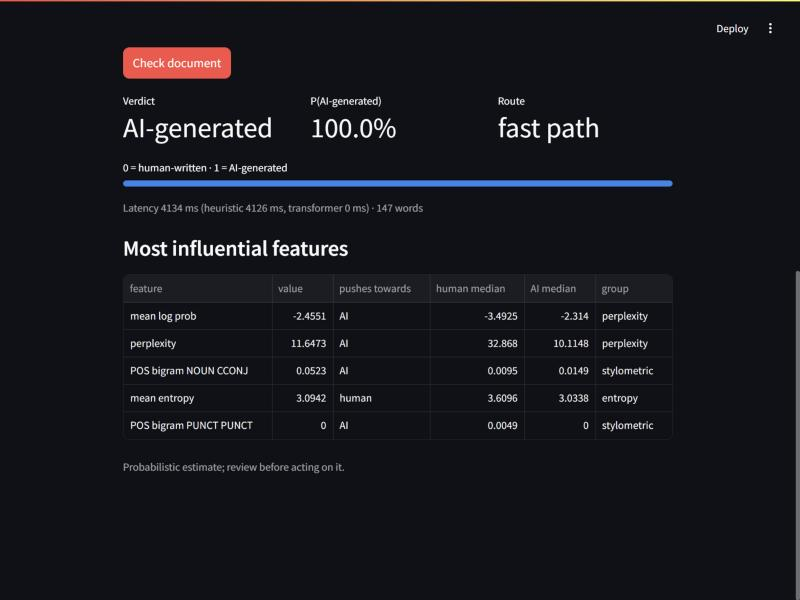
\includegraphics[width=0.82\textwidth]{web_ui_result.jpg}
\caption{Result panel of the web interface for an AI-generated test document}
\label{fig:webui}
\end{figure}

\subsection{Testing Strategy}

The test suite (34 tests, run with pytest) has three layers.
\textbf{Unit tests} check each module against hand-computed values: burstiness
is $-1$ for equal sentence lengths and $-1/3$ for lengths 5 and 15, the
type-token ratio is computed on the 200-word prefix only, the gate routes
probabilities exactly at the band edges (both edges escalate), the band search
finds the cheapest feasible band on synthetic data, the expected calibration
error is 0 for perfect and 1 for inverted predictions, and the bootstrap
interval contains the point estimate. \textbf{Integration tests} build a
complete cascade from stub models (a deterministic feature function in place
of GPT-2 and a keyword rule in place of RoBERTa), and check routing,
explanations, the ``insufficient text'' path, determinism, model
serialisation and that batch and single-document results agree. \textbf{API
tests} exercise every REST endpoint, including batch jobs from CSV and ZIP
uploads and the administrator token. A further test, marked as slow, runs the
real GPT-2 and spaCy feature extraction on a fixed paragraph.

% ---------------------------------------------------------------------
\section{Work Plan and Status}
% ---------------------------------------------------------------------

Fig.~\ref{fig:gantt} shows the work plan across the seventh and eighth
semesters. All implementation objectives (O1--O5) have been completed: the
data pipeline, both detection stages, the cascade with tuned operating points,
the full evaluation and the packaged command line tool, REST service and web
interface.

\begin{figure}[H]
\centering
\resizebox{\textwidth}{!}{%
\begin{tikzpicture}[x=1.05cm,y=0.62cm,font=\small]
  \foreach \m [count=\i] in {Aug,Sep,Oct,Nov,Dec,Jan,Feb,Mar,Apr}{
     \node[font=\small\bfseries] at (\i+0.5,0.8) {\m};
     \draw[gray!60] (\i,0.4) -- (\i,-10.6);
  }
  \draw[gray!60] (10,0.4) -- (10,-10.6);
  \node[font=\scriptsize] at (3.0,1.5) {2026};
  \node[font=\scriptsize] at (8.0,1.5) {2027};
  \foreach \y/\task/\s/\e/\done in {
      0/Literature survey/1/3.0/1,
      1/Problem formulation and objectives/2.5/3.5/1,
      2/Methodology and system design/3.0/4.5/1,
      3/Synopsis + paper + report (Ch. 1--6)/3.5/4.6/1,
      4/Data collection and corpus (O1)/4.5/4.7/1,
      5/Heuristic baseline (O1)/4.6/4.7/1,
      6/Transformer fine-tuning (O2)/4.6/4.7/1,
      7/Cascade and threshold tuning (O3)/4.65/4.75/1,
      8/Evaluation: LOGO and fairness (O4)/4.65/4.75/1,
      9/CLI + REST + web demo (O5)/4.55/4.75/1,
      10/Final report and viva/4.7/10.0/0}{
     \node[anchor=east] at (0.9,-\y) {\task};
     \ifnum\done=1
        \fill[black!70] (\s,-\y-0.3) rectangle (\e,-\y+0.3);
     \else
        \draw[thick,pattern=north east lines] (\s,-\y-0.3) rectangle (\e,-\y+0.3);
     \fi
  }
  \draw[very thick,dashed] (4.8,0.4) -- (4.8,-10.6) node[below,font=\scriptsize] {Nov 2026 (this report)};
  \fill[black!70] (1.0,-12.0) rectangle (1.6,-11.6); \node[anchor=west,font=\scriptsize] at (1.7,-11.8) {completed};
  \draw[thick,pattern=north east lines] (3.6,-12.0) rectangle (4.2,-11.6); \node[anchor=west,font=\scriptsize] at (4.3,-11.8) {remaining};
\end{tikzpicture}}
\caption{Project work plan and status (Gantt chart)}
\label{fig:gantt}
\end{figure}

\subsection{Differences Between the Plan and the Implementation}
\label{sec:deviations}

Table~\ref{tab:deviations} lists every point on which the implementation
differs from the plan described in Chapters~3--5 and in the earlier version of
this chapter, together with the reason. None of them changes the method; they
concern data availability, compute and one refinement of the fairness
constraint.

\begin{table}[H]
\caption{Differences between the planned and the implemented system}
\label{tab:deviations}
\centering
\small
\begin{tabularx}{\textwidth}{|p{3.4cm}|p{4.2cm}|L|}
\hline
\textbf{Item} & \textbf{Implemented} & \textbf{Reason} \\ \hline
Custom GPT-4, Claude and Llama generations & Generation script provided; not used in the reported corpus & API generations are billed per token; public benchmarks already contain GPT-4 and Llama texts \\ \hline
Held-out generator family & Mistral (RAID Mistral and Mistral-chat) & A modern family with enough texts that is absent from HC3 and M4, so it can be removed completely \\ \hline
Size of held-out and attack test sets & 744 and 690 documents instead of 2,000 & Limited by the number of test-split groups in the RAID sample \\ \hline
DeBERTa-v3 & Supported, not trained & RoBERTa-base already reached validation F1 0.981; GPU time was used for the second (leave-Llama-out) RoBERTa model instead \\ \hline
Hardware & Single local workstation (RTX 3060 Ti, 8 GB) & Sufficient for all runs with gradient accumulation; no data left the machine \\ \hline
Batch size & 4 per step $\times$ 4 accumulation steps & Same effective batch of 16 within 8 GB of GPU memory \\ \hline
Random seeds & One run (seed 42) & Compute time; bootstrap CIs are reported instead of seed variance \\ \hline
Fairness constraint & Worst-group form by default; disparity form available & The disparity-only form can be met by harming native writers (Chapter~\ref{ch:results}) \\ \hline
Fairness set length filter & Essays of all lengths scored & About a third of the TOEFL essays are shorter than 100 words; the deployed system would report them as ``insufficient text'' \\ \hline
NLTK & Not used & Function-word list is kept in the code \\ \hline
\end{tabularx}
\end{table}

\section{Summary}

This chapter described the implementation of \veriscript{}: the algorithms in
each module (reference-model scoring with GPT-2, spaCy segmentation and
tagging, logistic regression and XGBoost heads, Platt and isotonic calibration,
RoBERTa-base fine-tuning with AdamW, sliding-window inference and a vectorised
grid search over the ambiguity band), the software stack and the single
workstation on which all experiments ran, the searched and selected
hyperparameters and the latency measurement protocol. It described the corpus
of 44,618 documents built from HC3, M4, RAID, MAGE and the Liang \textit{et al.}
essays, with group-wise splits balanced by domain and length, and presented the
code organisation, key implementation excerpts, the training runs, the
interfaces and the test suite. The next chapter analyses the results against
the success criteria of Table~\ref{tab:gap-obj} and the hypotheses of
Chapter~\ref{ch:problem}.
